\documentclass[conference]{IEEEtran}
\IEEEoverridecommandlockouts
% The preceding line is only needed to identify funding in the first footnote. If that is unneeded, please comment it out.
\usepackage{cite}
\usepackage{amsmath,amssymb,amsfonts}
\usepackage{algorithmic}
\usepackage{graphicx}
\usepackage{textcomp}
\usepackage{xcolor}
\usepackage[brazilian]{babel}
\usepackage[utf8]{inputenc}
\usepackage[T1]{fontenc}
\usepackage{listings}
\usepackage{color}

\definecolor{dkgreen}{rgb}{0,0.6,0}
\definecolor{gray}{rgb}{0.5,0.5,0.5}
\definecolor{mauve}{rgb}{0.58,0,0.82}

\lstset{frame=tb,
  language=Java,
  aboveskip=3mm,
  belowskip=3mm,
  showstringspaces=false,
  columns=flexible,
  basicstyle={\small\ttfamily},
  numbers=none,
  numberstyle=\tiny\color{gray},
  keywordstyle=\color{blue},
  commentstyle=\color{dkgreen},
  stringstyle=\color{mauve},
  breaklines=true,
  breakatwhitespace=true,
  tabsize=3
}
\lstset{language=Python}
\def\BibTeX{{\rm B\kern-.05em{\sc i\kern-.025em b}\kern-.08em
    T\kern-.1667em\lower.7ex\hbox{E}\kern-.125emX}}
\begin{document}

\title{Relatório do Laboratório 2: \\ Busca Informada\\
}

\author{\IEEEauthorblockN{Isabelle Ferreira de Oliveira}
\IEEEauthorblockA{\textit{CT-213 - Engenharia da Computação 2020} \\
\textit{Instituto Tecnológico de Aeronáutica (ITA)}\\
São José dos Campos, Brasil \\
isabelle.ferreira3000@gmail.com}
}

\maketitle

\begin{abstract}
Esse relatório documenta a implementação de um planejador de caminho para um robô móvel, que está num determinado ambiente com obstáculos e quer encontrar um caminho até um objetivo. Foi implementado os algoritmos Dijkstra, Greedy Search e A* para realizar resolver esse problema de busca em grafos. Por fim, os resultados das três implementações foram comparados.
\end{abstract}

\begin{IEEEkeywords}
Planejamento de caminho, Dijkstra, Greedy, A*, robô móvel
\end{IEEEkeywords}

\section{Introdução}
Comportamentos autônamos de agentes podem ser implementados por diversos métodos atualmente. Entre esses métodos, pode-se organizar os possíveis comportamentos em Máquinas de Estados e Árvores de Comportamento (Behavior Trees).

Máquina de Estados é um modelo matemático para descrever um sistema. Nesse modelo, apenas um estado está sendo executado a cada momento e, para transitar entre um estado e outro, são necessários acontecimentos em específicos\cite{b1}. É possível representar o comportamento de um sistema descrito por Máquina de Estados por meio de um grafo direcionado, como o apresentado na Figura \ref{state_machine}.

Behavior Tree é outro modelo matemático também com a finalidade de descrever um sistema. Já nesse modelo, as folhas da árvore guardam os comportamentos mais básicos e os nós mais internos podem definir se os comportamentos básicos acontecerão em sequência, em ordem randômica, em paralelo, etc., acrescentando grau de complexidade aos comportamentos do agente. Após a execução de cada nó, é retornado Success (quando tarefa terminou com sucesso), Failure (quando tarefa falhou) ou Running (quando a tarefa deve continuar execução na próxima iteração) \cite{b1}. A representação de uma Behavior Tree pode ser vista na Figura \ref{behavior_tree}.

É possível modelar o comportamento de um robô de limpeza autônomo do tipo Roomba (desenvolvido pela empresa iRobot) a partir desses métodos descritos anteriormente, conforme foi descrito nesse relatório.

\section{Implementação de Estados}
Na parte relativa a implementação da máquina de estados, era necessário preencher os códigos das funções \textit{check\underline{\space}transition} e \textit{execute}, além do construtor das classes \textit{MoveForwardState}, \textit{MoveInSpiralState}, \textit{GoBackState} e \textit{RotateState}.

Para calcular quanto tempo já está sendo executado um determinado estado, foi adicionado nos respectivos construtores um contador que era acrescido cada vez que era executado o comportamento desse estado. Assim, o tempo seria esse contador vezes o tempo gasto em cada execução, conforme sugerido no roteiro do laboratório \cite{b1}.

As transições em cada estado foram implementadas nas respectivas funções \textit{check\underline{\space}transition} de cada classe de estado, conforme o apresentado na Figura \ref{state_machine}, retirado do roteiro do laboratório \cite{b1}.

\begin{figure}[htbp]
\centerline{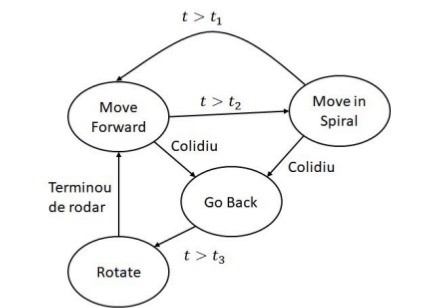
\includegraphics[scale=0.4]{maquina_estados.png}}
\caption{Máquina de estados finita do comportamento do Roomba.}
\label{state_machine}
\end{figure}

Já as funções \textit{execute}, além de realizarem o acréscimo do contador de execuções, também eram responsáveis por atualizar as velocidades do Roomba, a fim de que ele realizasse os movimentos esperados para cada estado. A ideia de cada uma das implementações também foi apresentada nas subseções abaixo, escritas em pseudo-Python.

Uma breve descrição em alto nível das implementações foi apresentada nas subsessões a seguir, com implementações escritas em pseudo-Python.

\subsection{Estado Move Forward}
Verificação das transições da máquina de estados na função \textit{check\underline{\space}transition} para o estado \textit{Move Forward}:
\begin{lstlisting}
if COLIDIU COM A PAREDE:
	MUDAR PARA ESTADO "GO BACK"
elif TEMPO_NESSE_ESTADO > TEMPO_NO_MOVE_FORWARD:
	MUDAR PARA ESTADO "MOVE IN SPIRAL"
\end{lstlisting}

Atualização das velocidades do Roomba na função \textit{execute} para o estado \textit{Move Forward}:
\begin{lstlisting}
ROOMBA.set_velocity(VELOCIDADE_LINEAR = FORWARD_SPEED, VELOCIDADE_ANGULAR = 0)
\end{lstlisting}

\subsection{Estado Move In Spiral}
Verificação das transições da máquina de estados na função \textit{check\underline{\space}transition} para o estado \textit{Move in Spiral}:
\begin{lstlisting}
if COLIDIU COM A PAREDE:
	MUDAR PARA ESTADO "GO BACK"
elif TEMPO_NESSE_ESTADO > TEMPO_NO_MOVE_IN_SPIRAL:
	MUDAR PARA ESTADO "MOVE FORWARD"
\end{lstlisting}

Atualização das velocidades do Roomba na função \textit{execute} para o estado \textit{Move In Spiral}:
\begin{lstlisting}
ROOMBA.set_velocity(VELOCIDADE_LINEAR = FORWARD_SPEED, VELOCIDADE_ANGULAR = FORWARD_SPEED/(INITIAL_RADIUS_SPIRAL + SPIRAL_FACTOR * TEMPO)
\end{lstlisting}

O cálculo dessa velocidade angular foi feito tendo em vista que o raio da espiral varia conforme a equação $r(t) = r_0 + b \cdot t$, onde $r_0$ é o raio inicial do espiral e $b$ é o fator do espiral, e que velocidade angular é velocidade linear dividido pelo raio da curva no instante.

\subsection{Estado Go Back}
Verificação das transições da máquina de estados na função \textit{check\underline{\space}transition} para o estado \textit{Go Back}:
\begin{lstlisting}
if TEMPO_NESSE_ESTADO > TEMPO_NO_GO_BACK:
	MUDAR PARA ESTADO "ROTATE"
\end{lstlisting}

Atualização das velocidades do Roomba na função \textit{execute} para o estado \textit{Go Back}:
\begin{lstlisting}
ROOMBA.set_velocity(VELOCIDADE_LINEAR = BACKWARD_SPEED, VELOCIDADE_ANGULAR = 0)
\end{lstlisting}

\subsection{Estado Rotate}
Verificação das transições da máquina de estados na função \textit{check\underline{\space}transition} para o estado \textit{Rotate}:
\begin{lstlisting}
if TEMPO_NESSE_ESTADO > TEMPO_NO_ROTATE:
	MUDAR PARA ESTADO "MOVE FORWARD"
\end{lstlisting}

O tempo que o Roomba passa no estado Rotate é calculado da seguinte maneira: um ângulo aleatório é escolhido entre $-\pi$ e $\pi$ para que ele faça a rotação e, dado a velocidade angular pré-estabelecida empregada nesse movimento, o tempo será o módulo desse ângulo dividido por essa velocidade.

Atualização das velocidades do Roomba na função \textit{execute} para o estado \textit{Go Back}:
\begin{lstlisting}
if ANGULO EH NEGATIVO:
	ROOMBA.set_velocity(VELOCIDADE_LINEAR = 0, VELOCIDADE_ANGULAR = -ANGULAR_SPEED)
else:
	ROOMBA.set_velocity(VELOCIDADE_LINEAR = 0, VELOCIDADE_ANGULAR = ANGULAR_SPEED)
\end{lstlisting}

\section{Implementação de Behaviors}
Já na parte relativa a implementação da Behavior Tree, era necessário preencher os códigos das funções \textit{enter} e \textit{execute}, além do construtor das classes \textit{RoombaBehaviorTree}, \textit{MoveForwardNode}, \textit{MoveInSpiralNode}, \textit{GoBackNode} e \textit{RotateNode}.

Para calcular quanto tempo já está sendo executado um determinado estado, foi feito de forma análoga ao feito na máquina de estados. Assim, foi adicionado nos construtores das classes folhas o contador que era acrescido cada vez que era executado o comportamento desse estado. Assim, o tempo também seria esse contador vezes o tempo gasto em cada execução.

Ao entrar em um Behavior, ou seja, na execução da função \textit{enter}, eram setadas as velocidades que permaneceriam constantes durante aquele behavior, além de serem zerados os contadores. No caso específico do behavior \textit{Move In Spiral}, como sua velocidade era alterada em cada instante, essa atualização da velocidade foi feita na função \textit{execute}.

\begin{figure}[htbp]
\centerline{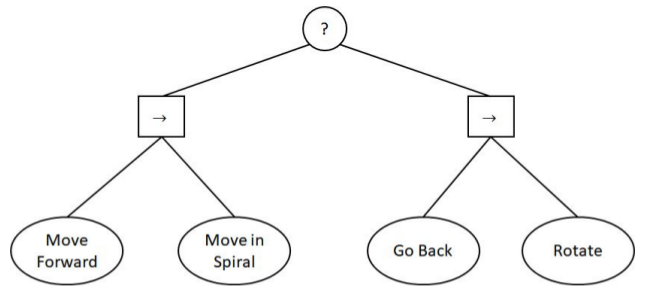
\includegraphics[scale=0.4]{behavior_tree.png}}
\caption{\textit{Behavior tree} do comportamento do Roomba.}
\label{behavior_tree}
\end{figure}

Já as funções \textit{execute}, além de realizarem o acréscimo do contador de execuções, também retornavam \textit{Success}, \textit{Failure} ou \textit{Running}, dependendo da situação que se encontrava o Roomba.

Uma breve descrição em alto nível das implementações foi apresentada nas subsessões a seguir, com implementações escritas em pseudo-Python.

\subsection{Roomba Behavior Tree}
A Behavior Tree precisou ser inicializada no construtor da classe \textit{RoombaBehaviorTree}. Sua implementação aconteceu fazendo de raiz o nó do tipo Selector, e adicionando como filhos da raiz dois nós do tipo Sequence. Por fim, foram adicionados nós folhas de cada behavior, conforme apresentado na Figura \ref{behavior_tree}. Dessa forma, a ideia de implementação, apresentada em pseudo-Python, foi apresentada abaixo.
\begin{lstlisting}
raiz = SelectorNode("root")

sequence_node_left = SequenceNode("left")
sequence_node_left.add_child(MoveForwardNode())
sequence_node_left.add_child(MoveInSpiralNode())

sequence_node_right = SequenceNode("right")
sequence_node_right.add_child(GoBackNode())
sequence_node_right.add_child(RotateNode())

raiz.add_child(sequence_node_left)
raiz.root.add_child(sequence_node_right)
\end{lstlisting}

\subsection{Behavior Move Forward}
Execução do behavior na função \textit{execute} para o estado \textit{Move Forward}:
\begin{lstlisting}
if TEMPO > TEMPO_NO_MOVE_FORWARD:
	return SUCCESS
if COLIDIU COM A PAREDE:
	return FAILURE
else:
	return RUNNING
\end{lstlisting}

Atualização das velocidades do Roomba na função \textit{enter} para o estado \textit{Move Forward}:
\begin{lstlisting}
ROOMBA.set_velocity(VELOCIDADE_LINEAR = FORWARD_SPEED, VELOCIDADE_ANGULAR = 0)
\end{lstlisting}

\subsection{Behavior Move In Spiral}
Execução do behavior na função \textit{execute} para o estado \textit{Move In Spiral}:
\begin{lstlisting}
if TEMPO > TEMPO_NO_MOVE_IN_SPIRAL:
	return SUCCESS
if COLIDIU COM A PAREDE:
	return FAILURE
else:
	return RUNNING
\end{lstlisting}

Atualização das velocidades do Roomba na função \textit{enter} para o estado \textit{Move In Spiral}:
\begin{lstlisting}
ROOMBA.set_velocity(VELOCIDADE_LINEAR = FORWARD_SPEED, VELOCIDADE_ANGULAR = FORWARD_SPEED / (INITIAL_RADIUS_SPIRAL + SPIRAL_FACTOR * TEMPO)
\end{lstlisting}

\subsection{Behavior Go Back}
Execução do behavior na função \textit{execute} para o estado \textit{Go Back}:
\begin{lstlisting}
if TEMPO > TEMPO_NO_GO_BACK:
	return SUCCESS
else:
	return RUNNING
\end{lstlisting}

Atualização das velocidades do Roomba na função \textit{enter} para o estado \textit{Go Back}:
\begin{lstlisting}
ROOMBA.set_velocity(VELOCIDADE_LINEAR = BACKWARD_SPEED, VELOCIDADE_ANGULAR = 0)
\end{lstlisting}

\subsection{Behavior Rotate}
Execução do behavior na função \textit{execute} para o estado \textit{Rotate}:
\begin{lstlisting}
if TEMPO > TEMPO_NO_ROTATE:
	return SUCCESS
else:
	return RUNNING
\end{lstlisting}

O tempo que o Roomba passa no estado Rotate e o ângulo que é rotacionado foram calculados de forma análoga ao que foi feito na implementação por máquina de estados.

Atualização das velocidades do Roomba na função \textit{enter} para o estado \textit{Rotate}:
\begin{lstlisting}
if ANGULO EH NEGATIVO:
	ROOMBA.set_velocity(VELOCIDADE_LINEAR = 0, VELOCIDADE_ANGULAR = -ANGULAR_SPEED)
else:
	ROOMBA.set_velocity(VELOCIDADE_LINEAR = 0, VELOCIDADE_ANGULAR = ANGULAR_SPEED)
\end{lstlisting}

\section{Resultados e Conclusões}
Os resultados obtidos após a implementação do comportamento do Roomba por meio de \textit{Máquina de Estados} foram apresentados nas Figuras \ref{test_state_machine_1} e \ref{test_state_mahine_2}; e por meio de \textit{Behavior Tree} nas Figuras \ref{test_behavior_tree_1} e \ref{test_behavior_tree_2}.

Foi possível notar que o comportamento do Roomba pode ser independentemente implementados por \textit{Máquina de Estados} e por \textit{Behavior Tree}. Suas simulações são inclusive idênticas até certo ponto, como pode-se observar a partir da comparação entre as Figuras \ref{test_state_machine_1} e Figura \ref{test_behavior_tree_1}.

\begin{figure}[htbp]
\centerline{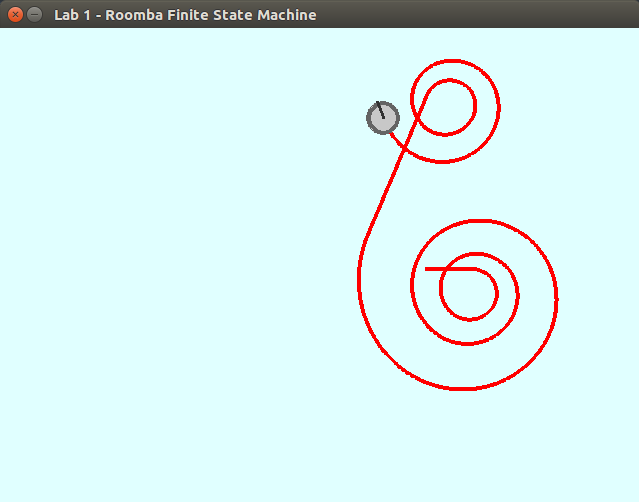
\includegraphics[scale=0.4]{test_state_machine_1.png}}
\caption{Simulação do Roomba para implementação por \textit{Máquina de Estados}. Na figura, é possível notar os estados Move Forward e Move In Spiral.}
\label{test_state_machine_1}
\end{figure}

\begin{figure}[htbp]
\centerline{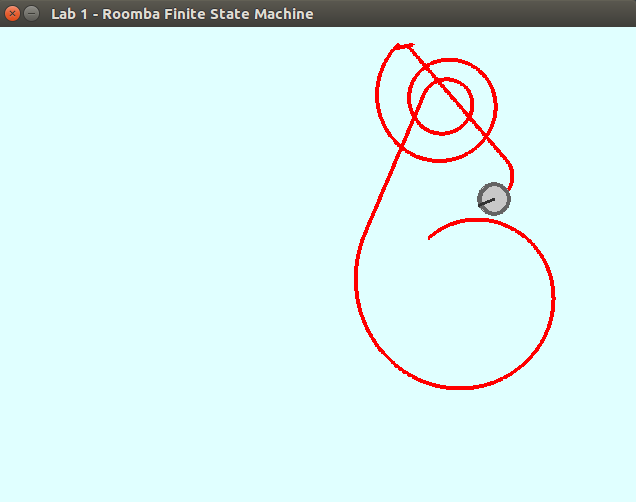
\includegraphics[scale=0.4]{test_state_machine_2.png}}
\caption{Simulação do Roomba para implementação por \textit{Máquina de Estados} segundos após a Figura \ref{test_state_machine_1}. Na figura, é possível notar os estados Move Forward, Move In Spiral, Go Back e Rotate.}
\label{test_state_mahine_2}
\end{figure} 

Isso era esperado, uma vez que, até o instante da imagem, a simulação tinha poucos segundos de execução, somente os estados/nós \textit{Move Forward} e \textit{Move In Spiral} tinham sido executados e nesses comportamentos não há nenhum fator que modifique os resultados independente das quantidade de vezes executadas.

Já para as Figuras \ref{test_state_mahine_2} e \ref{test_behavior_tree_2}, o Roomba já tinha sofrido pelo menos 1 colisão com a parede. Nesse instante, o robô executa o comportamento \textit{Go Back} e passa para o \textit{Rotate}, no qual um ângulo aleatório entre $-\pi$ e $\pi$ foi escolhido e rotacionado. 

Observou-se conforme o esperado que não há mais garantia que os movimentos sejam idênticos, dada a aleatoriedade dos ângulos. Para o caso da Figura \ref{test_state_mahine_2}, por exemplo, foram necessárias algumas colisões com a parede até que o Roomba consiga andar tempo suficiente para entrar no comportamento \textit{Move In Spiral}. Já no caso da Figura \ref{test_behavior_tree_2}, apenas uma colisão foi necessária. 



\begin{figure}[htbp]
\centerline{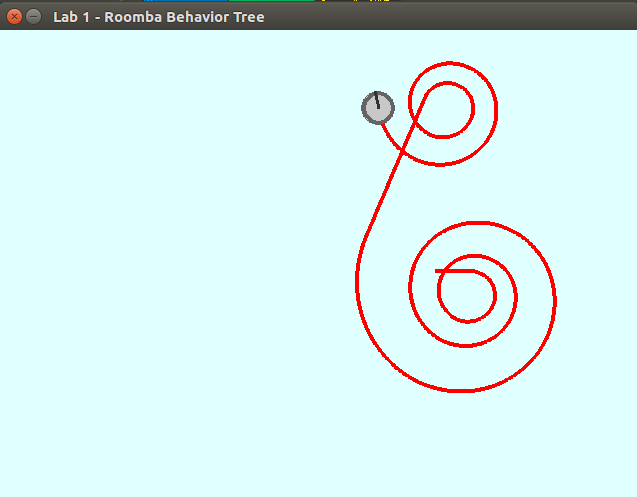
\includegraphics[scale=0.4]{test_behavior_tree_1.png}}
\caption{Simulação do Roomba para implementação por \textit{Behavior tree}. Na figura, é possível notar os estados Move Forward e Move In Spiral.}
\label{test_behavior_tree_1}
\end{figure}

\begin{figure}[htbp]
\centerline{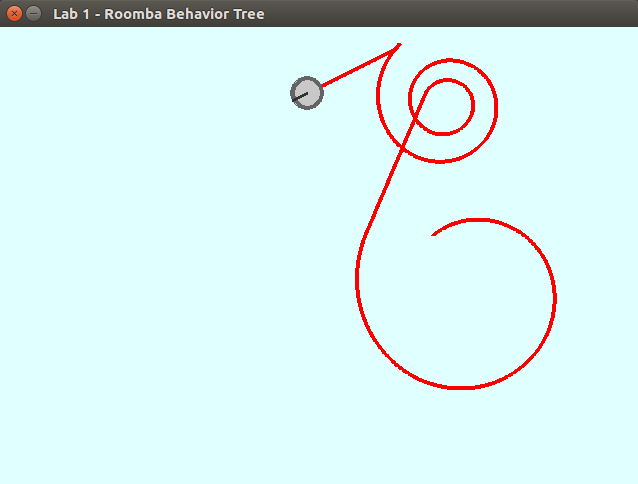
\includegraphics[scale=0.4]{test_behavior_tree_2.png}}
\caption{Simulação do Roomba para implementação por \textit{Behavior tree} segundos após a Figura \ref{test_behavior_tree_1}. Na figura, é possível notar os estados Move Forward, Move In Spiral, Go Back e Rotate.}
\label{test_behavior_tree_2}
\end{figure}

\begin{thebibliography}{00}
\bibitem{b1} M. Maximo, ``Roteiro: Laboratório 1 - Máquina de Estados Finita e Behavior Tree''. Instituto Tecnológico de Aeronáutica, Departamento de Computação. CT-213, 2019.
\end{thebibliography}

\end{document}
